\subsection{Commits to Revisions Mapping}

Translator performs translation of Git commits created by Git users into Subversion revisions, as well
as mirror translation of Subversion revisions created by Subversion users into Git commits. This section
describes how one concept (revision or commit) is mapped into another by Translator and how this mapping 
is stored.

\subsubsection{Git Commits to Subversion Revisions}

Every Git commit is translated to a single Subversion revision which modifies (or creates) a single branch or tag
in Subversion repository. Some of the non-commit changes, like Git branch or tag object creation are also translated into Subversion revisions.\\\\
\begin{figure}[!h]
\centering
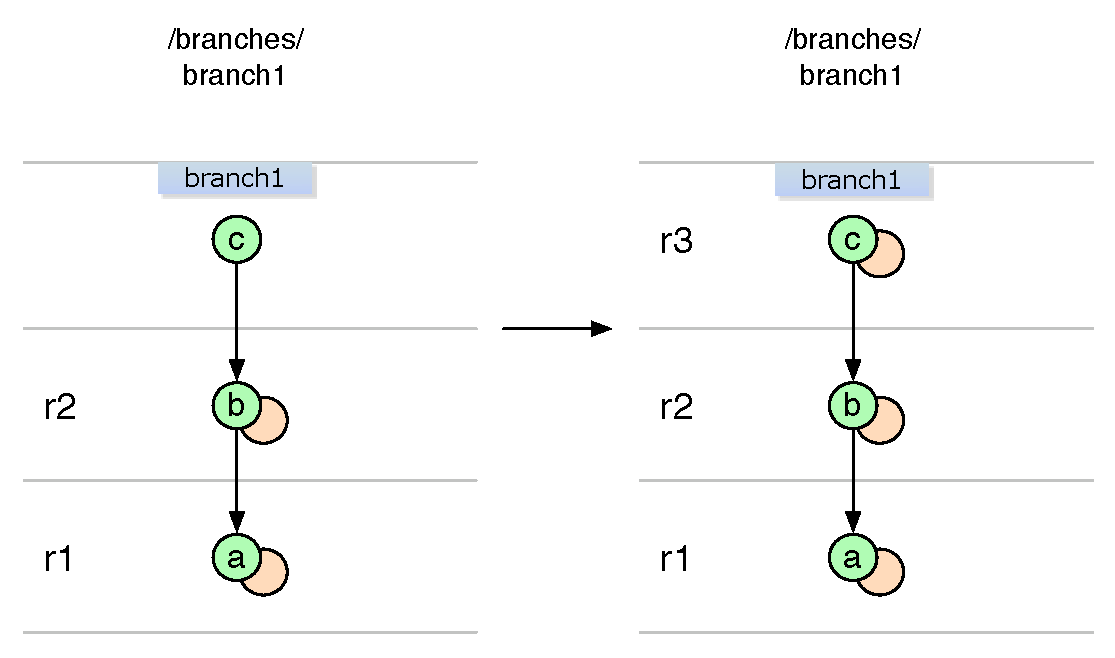
\includegraphics[width=\linewidth]{img/diagrams/single_change_git_to_svn.pdf}
\caption{Git Commit being translated to Subversion Revision}
\label{simple_git_to_svn}
\end{figure}Mapping between Git commit objects and corresponding revisions in Subversion repository (pair of revision number and branch name) is 
kept in Git repository, in a way similar to the one used to store Git notes. 
\\\\
Translator creates a special branch named /refs/mapping/svn and creates files in this branch named with Git commit object Id - this is the first part of the mapping. % S.: Not branch, but reference. Branch is something like /refs/heads/master or /refs/remote/origin/master.%
Contents of the file is Subversion revision number and branch name - second part of the mapping.
\\\\ 
By merging contents /.git/refs/mapping/svn branch to /.git/refs/notes we will get user friendly output of the mapping as part of the standard git log.

\subsubsection{Subversion Revisions to Git Commits}

Every Subversion revision is translated into one or more Git commits, depending on the amount of the branches affected by that particular Subversion commit.\\\\% S.: Maybe add a link to Branch and Tags subsection where all that stuff is considered? Maybe move all the diagrams from that section to the following one? And here just put references to them?%
Mapping between Subversion revision and corresponding Git commits is kept in Subversion repository in form of a special revision property.
\begin{figure}[!h]
\centering
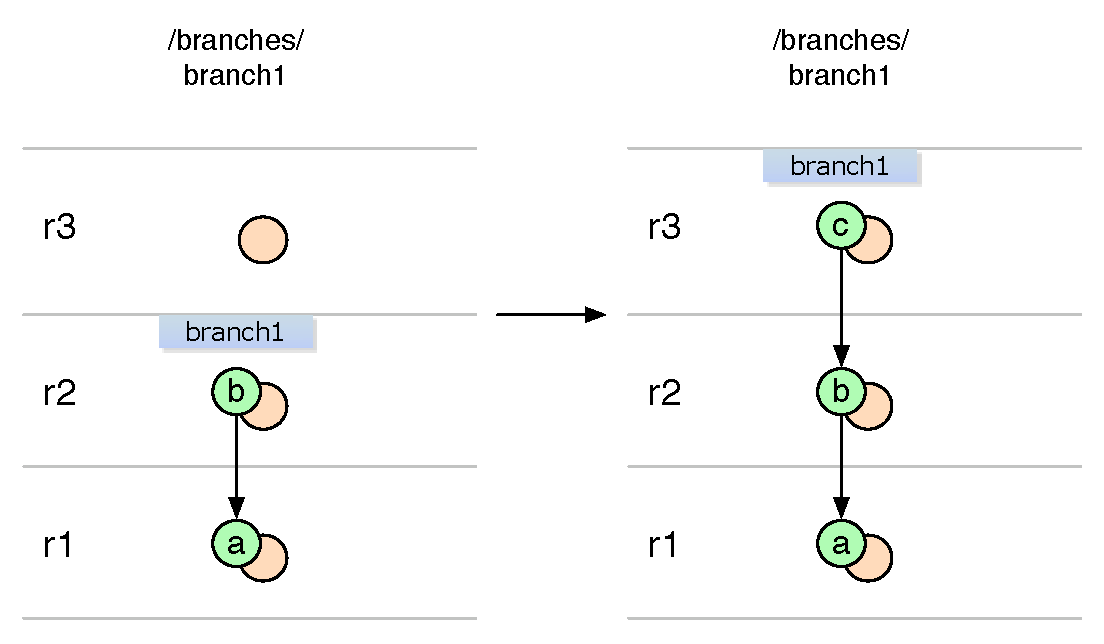
\includegraphics[width=\linewidth]{img/diagrams/single_change_svn_to_git.pdf}
\caption{Subversion Revision being translated to Git Commit}
\label{simple_svn_to_git}
\end{figure}
\\\\
Both mappings are kept in corresponding repositories (in a special branch and as revision properties), so that no special storage is needed. % S.: This mapping will be available for usual git and svn clients with no protocol changes.